\section{Three-term progressions under unit multipliers}
\label{sec:lemmaA}

The all-odd case of \autoref{sec:allodd} needs one purely arithmetic fact,
about how multiplication by a unit moves a short arithmetic progression
around the cycle $\Z/2k$. Cut $\Z/2k$ into the two halves $\{0,\dots,k-1\}$
and $\{k,\dots,2k-1\}$. Given odd $a<x$ with $x<k/2$, so that both lie in
the first quarter $\{0,\dots,k/2-1\}$ of the cycle,
is there a unit $\nu$ that sends $a$ and $2a-x$ to the same half and $x$ to
the other? Note that $2a-x$, $a$ and $x$ form a three-term progression with
difference $e=x-a$, so the question asks for a unit that separates the
progression after its middle term but not before it. Here I show that, when
$\gcd(a,x,k)=1$, the answer is yes at every even order $k>90$, with one
obvious exception.

The proof is by the geometry of numbers. The pairs $(\nu a,\nu e)$, reduced
modulo $2k$, are the points of a planar lattice of determinant $2k$, and a
lattice point with $\nu$ a unit in one of four open triangles yields a
witness. The triangles cover a quarter of the square $[0,2k)^2$, which
contains $2k$ lattice points, so one expects about $k/2$ lattice points in
them; the difficulty is to make this rigorous for every lattice, including
very skewed ones whose points lie on a few widely spaced lines, and to find a
unit point. Along a lattice line the multipliers form an arithmetic
progression, so Jacobsthal's function $J(n)$ bounds how far one must go
along a line to reach a unit. A short vector of the lattice then settles the
question: either it is long enough that a whole band of lines crosses the
incircle of a triangle, or it is one of finitely many short directions, for
which chords inside the triangles are tabulated once and for all. Above order
$2730$, elementary bounds on $J(n)$ and this chord table finish the proof
(\autoref{sec:lemmaA-tail}). At orders $92\le k\le2730$ with at most two
odd prime factors a direct argument applies (\autoref{sec:lemmaA-twoprime}),
and at the other orders up to $2730$ a finite certificate does
(\autoref{app:lemmaA-finite}). On a first reading one can skip the
proofs of the lemmas and \autoref{app:lemmaA-finite}.

\subsection{Statement}

The functions $H$ and $H_\nu$ are those of \eqref{eq:allodd-eps},
and witnesses and admissible triples are as in \autoref{def:allodd-adm}. For
an integer $y$ write $\langle y\rangle\in\{0,\dots,2k-1\}$ for its residue
modulo $2k$, so that $H(y)=1$ exactly when $\langle y\rangle<k$; recall also
that $H(y+k)=1-H(y)$, by \eqref{eq:allodd-flip}.

\begin{theorem}[three-term progressions]
\label{thm:lemmaA}
Every admissible triple $(k;a,x)$ with $k>90$ has a witness.
\end{theorem}

Both restrictions are genuine. If $x=3a$ then $2a-x=-a$, and since $\nu a$ is
odd it is neither $0$ nor $k$ modulo $2k$, so $H_\nu(-a)=
1-H_\nu(a)$ for every $\nu$. The bound on $k$ cannot simply be
dropped either: the triple $(90;1,33)$ satisfies every other condition, but
it has no witness, as a direct check of the $48$ units modulo $180$ shows.

It is convenient to work with the pair $(a,e)$, $e=x-a$, and to allow any
integer pair. Since $2a-x=a-e$ and $x=a+e$, a unit $\nu$ witnesses
$(k;A,A+E)$ exactly when
\begin{equation}
H\bigl(\nu(A-E)\bigr)=H(\nu A)\ne H\bigl(\nu(A+E)\bigr),
\label{eq:lemmaA-good}
\end{equation}
and I shall say that a pair $(A,E)$ of integers \emph{has a witness} if some
unit $\nu$ satisfies \eqref{eq:lemmaA-good}. Since $H$ depends only on residues
modulo $2k$, this depends only on $A$ and $E$ modulo $2k$.
\autoref{thm:lemmaA} states that $(a,x-a)$ has a witness.

Throughout the rest of the section $(k;a,x)$ is admissible with $k>90$,
unless stated otherwise, and $e=x-a$. Then
\begin{equation}
a\ \text{odd},\quad e\ \text{even},\quad 0<e,\quad a+e<k/2,\quad e\ne2a,
\quad \gcd(a,e,2k)=1.
\label{eq:lemmaA-adm}
\end{equation}
The last condition holds because a prime dividing $a$, $e$ and $2k$ is odd
(as $a$ is odd), so it divides $k$, $a$ and $x=a+e$.

\subsection{The target region}

The condition \eqref{eq:lemmaA-good} only involves the residues
$\langle \nu A\rangle$ and $\langle \nu E\rangle$, so it describes a region of the
square $[0,2k)^2$. It is enough to use four open triangles inside that region.
Let
\begin{align*}
\Delta_1&=\{(X,Y)\in\R^2:\ k/2<X<k,\ |Y-k/2|<X-k/2\}, & \Delta_2&=\Delta_1+(k,0),\\
\Delta_3&=\{(X,Y)\in\R^2:\ 0<X<k/2,\ |Y-3k/2|<k/2-X\}, & \Delta_4&=\Delta_3+(k,0),
\end{align*}
and $R=\Delta_1\cup \Delta_2\cup \Delta_3\cup \Delta_4\subset(0,2k)^2$. The triangle $\Delta_1$ has
vertices $(k/2,k/2)$, $(k,0)$ and $(k,k)$; it is right-angled and isosceles,
with legs $k/\sqrt2$ and hypotenuse $k$, so its inradius is
\begin{equation}
\rho=\tfrac12\bigl(k/\sqrt2+k/\sqrt2-k\bigr)=\tfrac12(\sqrt2-1)\,k,
\label{eq:lemmaA-rho}
\end{equation}
and its incentre is $O=(k-\rho,k/2)$. The other three triangles are
congruent to it. \autoref{fig:lemmaA-geometry} shows the four triangles
inside the square, together with the lattice of the next subsection.

\begin{figure}
\centering
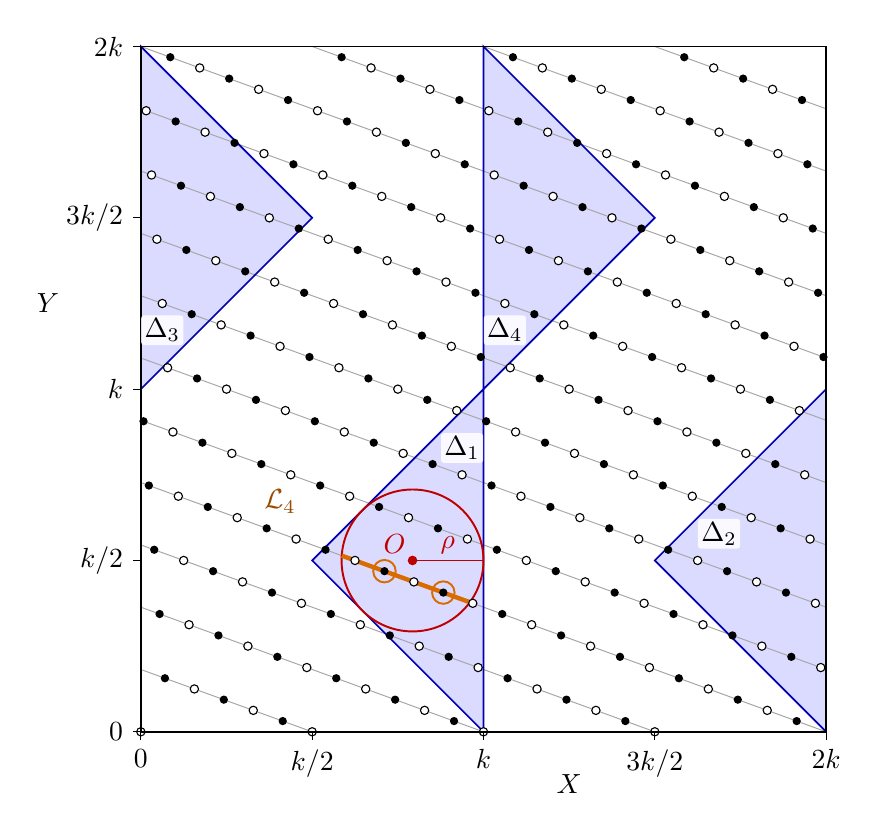
\begin{tikzpicture}[x=0.034cm,y=0.034cm,
  pt/.style={circle,inner sep=0pt,minimum size=3pt},
  lab/.style={fill=white,fill opacity=0.85,text opacity=1,
    inner sep=1.2pt,rounded corners=1pt}]
  % target region R: Delta_1, ..., Delta_4 (k = 128)
  \fill[blue!14] (64,64) -- (128,0) -- (128,128) -- cycle;
  \fill[blue!14] (192,64) -- (256,0) -- (256,128) -- cycle;
  \fill[blue!14] (0,128) -- (0,256) -- (64,192) -- cycle;
  \fill[blue!14] (128,128) -- (128,256) -- (192,192) -- cycle;
  % lattice lines \mathcal L_j = j w + t v, w = (9,20), v = (11,-4)
  \begin{scope}
    \clip (0,0) rectangle (256,256);
    \foreach \j in {0,...,14}
      \draw[black!35,line width=0.35pt]
        ({9*\j-11*10},{20*\j+4*10}) -- ({9*\j+11*21},{20*\j-4*21});
  \end{scope}
  \begin{scope}[blue!70!black,line width=0.6pt]
    \draw (64,64) -- (128,0) -- (128,128) -- cycle;
    \draw (192,64) -- (256,0) -- (256,128) -- cycle;
    \draw (0,128) -- (0,256) -- (64,192) -- cycle;
    \draw (128,128) -- (128,256) -- (192,192) -- cycle;
  \end{scope}
  % incircle D of Delta_1, centre O = (k - rho, k/2), rho = (sqrt2 - 1) k / 2
  \draw[red!75!black,line width=0.7pt] (101.490,64) circle (26.510);
  % chord of \mathcal L_4 across D
  \draw[orange!85!black,line width=1.6pt] (75.04,65.80) -- (122.92,48.39);
  % lattice points (<9d>, <20d>), d = 0, ..., 2k - 1; units are the odd d
  \foreach \d in {0,...,255} {
    \pgfmathtruncatemacro\X{mod(9*\d,256)}
    \pgfmathtruncatemacro\Y{mod(20*\d,256)}
    \ifodd\d
      \node[pt,fill=black] at (\X,\Y) {};
    \else
      \node[pt,draw=black,fill=white,line width=0.4pt] at (\X,\Y) {};
    \fi
  }
  % the two unit points of the chord, d = 67 and d = 41
  \foreach \P in {(91,60),(113,52)}
    \draw[orange!85!black,line width=0.7pt] \P circle (4.2);
  % centre and radius
  \draw[red!75!black,line width=0.6pt] (101.490,64) -- (128,64);
  \fill[red!75!black] (101.490,64) circle (1.8);
  \node[red!75!black,above left=-1pt] at (101.490,64) {$O$};
  \node[red!75!black,above=-1pt] at (114.7,64) {$\rho$};
  % frame and ticks
  \draw[line width=0.6pt] (0,0) rectangle (256,256);
  \foreach \t/\s in {0/0,64/{k/2},128/k,192/{3k/2},256/2k} {
    \draw (\t,0) -- (\t,-3) node[below] {$\s$};
    \draw (0,\t) -- (-3,\t) node[left] {$\s$};
  }
  \node[below=12pt] at (160,0) {$X$};
  \node[left=26pt] at (0,160) {$Y$};
  % labels
  \node[lab] at (120,106) {$\Delta_1$};
  \node[lab] at (216,74) {$\Delta_2$};
  \node[lab] at (8,150) {$\Delta_3$};
  \node[lab] at (136,150) {$\Delta_4$};
  \node[text=orange!60!black,inner sep=0pt] at (52,86) {$\mathcal L_4$};
\end{tikzpicture}
\caption{The geometry of \autoref{lem:lemmaA-region} and
\autoref{prop:lemmaA-band}, drawn to scale for $k=128$ and $(a,e)=(9,20)$.
The square is $[0,2k]^2$ and the shaded triangles are $\Delta_1,\dots,\Delta_4$. The
dots are the $2k$ points $(\langle \nu a\rangle,\langle \nu e\rangle)$ of
$\Lambda$ in the square, filled for the unit points ($\nu$ odd) and open for
the others. A shortest vector is $v=(11,-4)$, of length $l=\sqrt{137}$, and
$w=(a,e)$ has $v\times w=2k$; the grey lines are the lines
$\mathcal L_0,\dots,\mathcal L_{14}$, a distance $2k/l\approx21.9$ apart. The circle is the
incircle of $\Delta_1$, with centre $O$ and radius $\rho$. The line $\mathcal L_4$ passes
within $0.06\,k$ of $O$, and its chord across the disc (thick) contains
the points with $\nu=208,67,182,41$; the two unit points among them (circled)
show that $(9,20)$ has a witness. Here $g=1$ and $n=2$, and both hypotheses of
\autoref{prop:lemmaA-band} hold.}
\label{fig:lemmaA-geometry}
\end{figure}

\begin{lemma}[the target region]
\label{lem:lemmaA-region}
If $\gcd(\nu,2k)=1$ and $(\langle \nu A\rangle,\langle \nu E\rangle)\in R$, then
$\nu$ satisfies \eqref{eq:lemmaA-good}, so $(A,E)$ has a witness.
\end{lemma}

\begin{proof}
Write $X=\langle \nu A\rangle$ and $Y=\langle \nu E\rangle$, so that
$H(\nu A)=H(X)$ and $H(\nu(A\pm E))=H(X\pm Y)$. If $(X,Y)\in \Delta_1$ then
$k-X<Y<X$, so $0<X-Y<2X-k<k$ and $k<X+Y<2X<2k$; hence
$H(X-Y)=1=H(X)$ and $H(X+Y)=0$. If $(X,Y)\in \Delta_3$ then $k+X<Y<2k-X$, so
$X-Y$ lies in $(2X-2k,-k)$, which is $(2X,k)$ modulo $2k$, and $X+Y$ lies in
$(k+2X,2k)$; hence again $H(X-Y)=1=H(X)$ and $H(X+Y)=0$. Finally, replacing
$X$ by $X+k$ adds $k$ to each of $X$ and $X\pm Y$, which reverses all three
values of $H$ and so preserves the pattern $H(X-Y)=H(X)\ne H(X+Y)$. This
covers $\Delta_2$ and $\Delta_4$.
\end{proof}

\subsection{The lattice}

The pairs $(\nu a,\nu e)$ modulo $2k$ are the points of a lattice. It is
simplest to define it by a single congruence:
\[
\Lambda=\{w=(w_1,w_2)\in\Z^2:\ 2k\mid w_1e-w_2a\}.
\]
Since $\gcd(a,e,2k)=1$, fix integers $\xi_1,\xi_2,\xi_3$ with
$\xi_1 a+\xi_2 e+2k\xi_3=1$, and define the \emph{label} of $w\in\Z^2$ as
$\lambda(w)=\xi_1 w_1+\xi_2 w_2$. For $w,w'\in\R^2$ write
$w\times w'=w_1w_2'-w_2w_1'$ and $w\cdot w'$ for the dot product.

\begin{lemma}[labels]
\label{lem:lemmaA-labels}
\begin{enumerate}
\item[(a)] $\Lambda$ is a subgroup of $\Z^2$ containing $2k\Z^2$ and
$(\nu a,\nu e)$ for every $\nu\in\Z$, and every $w\in\Lambda$ satisfies
$w\equiv\lambda(w)\,(a,e)\pmod{2k}$. In particular
$\Lambda=\Z(a,e)+2k\Z^2$, and $\lambda$ is additive.
\item[(b)] If $w,w'\in\Lambda$ then $2k\mid w\times w'$.
\item[(c)] If $w\in\Lambda$, $\gcd(\lambda(w),2k)=1$ and
$(\langle w_1\rangle,\langle w_2\rangle)\in R$, then $(a,e)$ has a witness.
\end{enumerate}
\end{lemma}

\begin{proof}
(a) The first claims are clear. If $w_1e-w_2a=2kc$ then
\[
w_1-\lambda(w)a=w_1(\xi_2 e+2k\xi_3)-\xi_2 aw_2=\xi_2\cdot2kc+2k\xi_3 w_1,
\]
and similarly $w_2-\lambda(w)e=-\xi_1\cdot2kc+2k\xi_3 w_2$.
(b) By (a), $w\times w'\equiv\lambda(w)\lambda(w')\,(a,e)\times(a,e)=0$
modulo $2k$. (c) By (a), $\langle\lambda(w)a\rangle=\langle w_1\rangle$ and
$\langle\lambda(w)e\rangle=\langle w_2\rangle$, so
\autoref{lem:lemmaA-region} applies with $\nu=\lambda(w)$.
\end{proof}

Call $w\in\Lambda$ a \emph{unit point} if $\gcd(\lambda(w),2k)=1$. By
\autoref{lem:lemmaA-labels}(c), the task is to find a unit point of $\Lambda$
in $R+2k\Z^2$. The next lemma collects what a shortest vector of $\Lambda$
provides; part (b) is Hermite's bound in dimension two.

\begin{lemma}[a shortest vector]
\label{lem:lemmaA-frame}
Let $v$ be a nonzero vector of $\Lambda$ of least Euclidean length
$l=|v|$, let $g=\gcd(v_1,v_2)$ and $u=(p,q)=v/g$. Then:
\begin{enumerate}
\item[(a)] there is $w\in\Lambda$ with $v\times w=2k$;
\item[(b)] $3l^4\le16k^2$;
\item[(c)] $g\mid2k$, $gq$ is even, and $mu\notin\Lambda$ for $0<m<g$;
\item[(d)] $g\mid\lambda(v)$, and every common divisor of $\lambda(v)$ and
$2k$ divides $g$;
\item[(e)] $\gcd(\lambda(w),g)=1$ for every $w$ as in (a).
\end{enumerate}
\end{lemma}

\begin{proof}
(a) Write $v_1e-v_2a=2k\varphi$ and $c=\gcd(v_1,v_2,\varphi)$. Then
$v/c\in\Lambda$ is nonzero, so $c=1$ by minimality. Take integers
$\mu_1,\mu_2,\mu_3$ with $\mu_1v_1+\mu_2v_2+\mu_3\varphi=1$ and put
$w=(-2k\mu_2+\mu_3a,\ 2k\mu_1+\mu_3e)$. Then $w\in\Lambda$ (it is
$\mu_3(a,e)$ plus a vector of $2k\Z^2$), and
$v\times w=2k(\mu_1v_1+\mu_2v_2)+\mu_3(v_1e-v_2a)=2k$.

(b) Replacing $w$ by $w+tv$ with $t\in\Z$ does not change $v\times w$, so I
may assume $|v\cdot w|\le l^2/2$. Since $w\ne0$, $|w|\ge l$. Lagrange's
identity $(v\times w)^2+(v\cdot w)^2=|v|^2|w|^2$ gives
$4k^2\ge l^4-l^4/4$.

(c) Let $g'=\gcd(2k,g)=\zeta_12k+\zeta_2g$. Then $g'u=\zeta_1(2ku)+\zeta_2v\in\Lambda$
is nonzero, so $g'|u|\ge l=g|u|$, and $g'=g$; thus $g\mid2k$. If $0<m<g$ then
$mu$ is nonzero and shorter than $v$, so $mu\notin\Lambda$. Finally
$v_2a\equiv v_1e\pmod{2k}$ with $e$ and $2k$ even, so $v_2a$ is even, and
since $a$ is odd, $v_2=gq$ is even.

(d) $\lambda(v)=g(\xi_1 p+\xi_2 q)$. If $c$ divides $\lambda(v)$ and $2k$,
then by \autoref{lem:lemmaA-labels}(a) it divides $v_1$ and $v_2$, hence $g$.

(e) For every $z\in\R^2$, $(v\times w)\,z=(z\times w)\,v+(v\times z)\,w$
(both sides are linear in $z$ and agree at $z=v$ and $z=w$). Take
$z=(a,e)\in\Lambda$: by \autoref{lem:lemmaA-labels}(b) both $z\times w$ and
$v\times z$ are multiples of $2k=v\times w$, so $(a,e)=c_1v+c_2w$ with
$c_1,c_2\in\Z$. Applying the additive map $\lambda$,
$1-2k\xi_3=\xi_1 a+\xi_2 e=c_1\lambda(v)+c_2\lambda(w)$. Since $g$ divides
$2k$ and $\lambda(v)$, it is prime to $\lambda(w)$.
\end{proof}

Replacing $(v,w)$ by $(-v,-w)$ changes none of these properties, so I may
and do assume that $u$ is \emph{normalised}: $p>0$, or $p=0<q$. Eight short
directions never occur.

\begin{lemma}[eight excluded directions]
\label{lem:lemmaA-zero}
With $v=gu$ as in \autoref{lem:lemmaA-frame} and $u=(p,q)$ normalised,
$(g;p,q)$ is none of
\[
(1;1,0),\ (1;1,2),\ (2;0,1),\ (2;1,0),\ (2;1,1),\ (2;1,-1),\ (2;1,-2),\
(4;0,1).
\]
\end{lemma}

\begin{proof}
Each case says that $2k$ divides $g(pe-qa)$, and each contradicts
\eqref{eq:lemmaA-adm}. For $(1;1,0)$: $2k\mid e$, but $0<e<k$.
For $(1;1,2)$: $2k\mid e-2a$ with $|e-2a|<k$, so $e=2a$. For $(2;0,1)$:
$k\mid a$, but $0<a<k$. For $(2;1,0)$: $k\mid e$. For $(2;1,\pm1)$:
$k\mid e\mp a$, which is odd while $k$ is even. For $(2;1,-2)$: $k\mid e+2a$,
but $0<e+2a=x+a<k$. For $(4;0,1)$: $k/2\mid a$, but $0<a<k/2$.
\end{proof}

\subsection{Lattice lines and Jacobsthal's function}
\label{sec:lemmaA-jac}

For $n\ge1$, \emph{Jacobsthal's function} $J(n)$ is the least $m$ such that
every $m$ consecutive integers include one prime to $n$
\citep{Jacobsthal1960a,Jacobsthal1960b,Jacobsthal1960c}. It depends only on
the set of primes dividing $n$, and $J(n')\le J(n)$ whenever every prime
factor of $n'$ divides $n$. Deep asymptotic bounds are known, such as
$J(n)\ll\omega(n)^2\log^2\omega(n)$, with $\omega(n)$ the number of
distinct prime factors of $n$ \citep{Iwaniec1978}, but the elementary bounds
proved below suffice here.

Fix $v=gu$ and $w$ as in \autoref{lem:lemmaA-frame}, and write
$\lambda_v=\lambda(v)$ and $\lambda_w=\lambda(w)$. For $j\in\Z$ let
\[
\mathcal L_j=\{jw+tv:\ t\in\R\}
\]
(see \autoref{fig:lemmaA-geometry}).
Since $v\times(jw+tv)=2kj$, the line $\mathcal L_j$ lies at signed distance
$2kj/l$ from $\mathcal L_0$; consecutive lines are $2k/l$ apart. The points
$jw+iv$ with $i\in\Z$ lie in $\Lambda$, a distance $l$ apart, and their
labels $j\lambda_w+i\lambda_v$ form an arithmetic progression.

\begin{lemma}[unit points on a line]
\label{lem:lemmaA-line}
Let $n\ge1$ divide $2k$, with $\gcd(n,g)=1$ and every prime factor of $2k$
dividing $n$ or $g$ (for instance, $n$ the product of the primes of $2k$
that do not divide $g$). If $\gcd(j,g)=1$, then among any $J(n)$ consecutive
points $jw+iv$ of $\mathcal L_j$ there is a unit point.
\end{lemma}

\begin{proof}
A common divisor of $\lambda_v$ and $n$ divides $2k$, so it divides $g$ by
\autoref{lem:lemmaA-frame}(d), and it is $1$ since $\gcd(n,g)=1$. Choose
$\iota$ with $\iota\lambda_v\equiv1\pmod n$. Then
$j\lambda_w+i\lambda_v\equiv\lambda_v(i+\iota j\lambda_w)\pmod n$, and as $i$ runs
through $J(n)$ consecutive integers so does $i+\iota j\lambda_w$; so for one
of them $j\lambda_w+i\lambda_v$ is prime to $n$. A prime $\ell$ dividing $g$
divides $\lambda_v$ (\autoref{lem:lemmaA-frame}(d)) but neither $j$ nor
$\lambda_w$ (\autoref{lem:lemmaA-frame}(e)), so it does not divide
$j\lambda_w+i\lambda_v$. Every prime of $2k$ divides $n$ or $g$, so this label is
prime to $2k$.
\end{proof}

\begin{lemma}[chords]
\label{lem:lemmaA-chord}
Let $n$ be as in \autoref{lem:lemmaA-line}, $\gcd(j,g)=1$, $\Delta$ one of
$\Delta_1,\dots,\Delta_4$ and $z\in\Z^2$. If $t_0<t_1$, $t_1-t_0>J(n)$ and
$jw+tv\in\Delta+2kz$ for all $t\in(t_0,t_1)$, then $(a,e)$ has a witness.
\end{lemma}

\begin{proof}
The integers $i_0,\dots,i_0+J(n)-1$ with $i_0=\lfloor t_0\rfloor+1$ lie in
$(t_0,t_0+J(n)]\subset(t_0,t_1)$. By \autoref{lem:lemmaA-line} one of the
points $jw+iv$ with such $i$ is a unit point. It lies in $\Delta+2kz$, and since
$\Delta\subset(0,2k)^2$ its residues modulo $2k$ lie in $\Delta\subset R$. Now apply
\autoref{lem:lemmaA-labels}(c).
\end{proof}

\subsection{Two ways to find a chord}

The first way uses a band of lines through the incircle of $\Delta_1$, and works
when the shortest vector is long.

\begin{proposition}[the band]
\label{prop:lemmaA-band}
With $v=gu$ as in \autoref{lem:lemmaA-frame} and $n$ as in
\autoref{lem:lemmaA-line}, suppose that
\[
J(g)<0.102\,l\qquad\text{and}\qquad J(n)\,l<0.3604\,k.
\]
Then $(a,e)$ has a witness.
\end{proposition}

\begin{proof}
Let $D$ be the open disc of radius $\rho$ about the incentre $O$ of $\Delta_1$;
it lies in $\Delta_1$. Put $\tau=(v\times O)/2k$, so that $O$ is at signed
distance $2k\tau/l$ from $\mathcal L_0$. The $J(g)$ consecutive integers
$\lfloor\tau-J(g)/2\rfloor+1,\dots,\lfloor\tau-J(g)/2\rfloor+J(g)$ include
one, $j$, prime to $g$, and every one of them satisfies $|j-\tau|\le J(g)/2$.
So the distance from $O$ to $\mathcal L_j$ is at most
$(2k/l)\,J(g)/2=J(g)k/l<0.102\,k$. The line $\mathcal L_j$ therefore meets $D$
in an open segment of length greater than $2\sqrt{\rho^2-(0.102\,k)^2}$. By
\eqref{eq:lemmaA-rho}, $\rho^2=\tfrac14(3-2\sqrt2)k^2>0.04289\,k^2$, and
$(0.102\,k)^2=0.010404\,k^2$, so the segment is longer than
$2\sqrt{0.03248}\,k>0.3604\,k>J(n)\,l$. In terms of the parameter $t$ of
$\mathcal L_j$ (in which the lattice points sit at the integers) the segment has
length greater than $J(n)$, and it lies in $\Delta_1$.
\autoref{lem:lemmaA-chord} completes the proof.
\end{proof}

The second way handles the short directions. Its key feature is that the
geometry does not depend on $k$, $a$ or $e$ once everything is scaled by
$2k$. Scale the triangles: let $\widehat\Delta_i=\Delta_i/2k$, so that
\begin{align*}
\widehat\Delta_1&=\{(X,Y):\ \tfrac14<X<\tfrac12,\ |Y-\tfrac14|<X-\tfrac14\}, &
\widehat\Delta_2&=\widehat\Delta_1+(\tfrac12,0),\\
\widehat\Delta_3&=\{(X,Y):\ 0<X<\tfrac14,\ |Y-\tfrac34|<\tfrac14-X\}, &
\widehat\Delta_4&=\widehat\Delta_3+(\tfrac12,0).
\end{align*}
For a primitive $u=(p,q)$, an integer $g\ge1$ and $j\in\Z$, consider the
line
\[
\widehat{\mathcal L}_j(g,u)=\Bigl\{\frac{j}{g|u|^2}\,(-q,p)+s\,u:\ s\in\R\Bigr\}.
\]
If $v=gu$ and $w$ are as in \autoref{lem:lemmaA-frame}, then
$(-q,p)\cdot w=u\times w=2k/g$, and decomposing $w$ along $u$ and $(-q,p)$
gives
\begin{equation}
\frac{jw+tv}{2k}=\frac{j}{g|u|^2}\,(-q,p)+\Bigl(s_*+\frac{g}{2k}\,t\Bigr)u,
\qquad s_*=\frac{j\,(u\cdot w)}{2k|u|^2}.
\label{eq:lemmaA-scaled}
\end{equation}
So $\mathcal L_j/2k=\widehat{\mathcal L}_j(g,u)$, and a change of $s$ by $\psi$ is a change of $t$ by
$2k\psi/g$.

\begin{definition}
\label{def:lemmaA-witness}
A \emph{chord witness} for $(g;p,q)$ consists of an integer $j$ with
$\gcd(j,g)=1$, an index $i\in\{1,2,3,4\}$, a vector $z\in\Z^2$ and rationals
$s_0<s_1$ such that the point of $\widehat{\mathcal L}_j(g,u)$ with parameter $s$ lies in
$\widehat\Delta_i+z$ for every $s\in(s_0,s_1)$. Its \emph{length} is
$\psi=s_1-s_0$.
\end{definition}

A chord witness is checked by evaluating finitely many signs. Each
$\widehat\Delta_i+z$ is the intersection of three open half-planes $\{f>0\}$ with
$f$ affine. If, for each of the three functionals, $f\ge0$ at the two points
with parameters $s_0$ and $s_1$ and $f>0$ at one of them, then $f>0$ on the
open segment between them, because along the segment $f$ is a combination
of its two end values with positive weights. These are nine rational sign
conditions.

\begin{proposition}[a tabulated chord]
\label{prop:lemmaA-table}
With $v=gu$ as in \autoref{lem:lemmaA-frame} and $n$ as in
\autoref{lem:lemmaA-line}, suppose $(g;p,q)$ has a chord witness of length
$\psi$ with $2k\psi>J(n)\,g$. Then $(a,e)$ has a witness.
\end{proposition}

\begin{proof}
By \eqref{eq:lemmaA-scaled}, $jw+tv\in\Delta_i+2kz$ for all $t$ in an open
interval of length $2k\psi/g>J(n)$. \autoref{lem:lemmaA-chord} applies.
\end{proof}

When neither proposition applies directly, the lattice can be pinned down
completely. Since $gu\in\Lambda$, the pair $(a,e)$ is, up to a unit, one of
at most $g^2$ explicit pairs.

\begin{lemma}[lattice classes]
\label{lem:lemmaA-class}
Let $v=gu$ be as in \autoref{lem:lemmaA-frame} and $n_0=2k/g$. There are a
unit $\eta$ modulo $2k$ and integers $0\le s,t<g$ (unrelated to the line
parameters above) such that, with
$(A,E)=(p+n_0s,\,q+n_0t)$,
\[
\eta\,(a,e)\equiv(A,E)\pmod{2k}.
\]
Moreover $\gcd(A,E,2k)=1$, and $2k\nmid m(pE-qA)$ for $0<m<g$. In
particular, if $(A,E)$ has a witness then so does $(a,e)$.
\end{lemma}

\begin{proof}
By \autoref{lem:lemmaA-frame}(d), $\lambda_v=\lambda(v)=g\lambda^*$, and
$\gcd(\lambda^*,n_0)=1$: if $c$ divides both then $gc$ divides $2k$ and
$\lambda_v$, hence $g$, so $c=1$. By \autoref{lem:lemmaA-labels}(a),
$g(p,q)=v\equiv g\lambda^*(a,e)\pmod{2k}$, so
$\lambda^*(a,e)\equiv(p,q)\pmod{n_0}$. Every unit modulo $n_0$ lifts to a
unit modulo $2k$: take $\eta=\lambda^*+n_0r$, with $r$ the product of the
primes of $2k$ that divide neither $n_0$ nor $\lambda^*$. Indeed, let $\ell$ be
a prime dividing $2k$. If $\ell\mid n_0$, then $\eta\equiv\lambda^*\not\equiv0
\pmod\ell$, as $\gcd(\lambda^*,n_0)=1$. If $\ell\nmid n_0$ and
$\ell\mid\lambda^*$, then $\ell\nmid r$, and $\eta\equiv n_0r\not\equiv0$. If
$\ell$ divides neither, then $\ell\mid r$, and $\eta\equiv\lambda^*\not\equiv0$. Then
$\eta a=p+n_0K_1$ and $\eta e=q+n_0K_2$ for some integers $K_1,K_2$, and
with $s,t$ the residues of $K_1,K_2$ modulo $g$ one gets
$\eta(a,e)\equiv(A,E)\pmod{n_0g}$, as claimed.

If $c$ divides $A$, $E$ and $2k$, it divides $\eta a$ and $\eta e$, hence
$\eta(\xi_1 a+\xi_2 e+2k\xi_3)=\eta$, and $c=1$. If $2k\mid m(pE-qA)$, then
$2k\mid m\eta(pe-qa)$, so $2k\mid m(pe-qa)$, that is $mu\in\Lambda$; this is
impossible for $0<m<g$ by \autoref{lem:lemmaA-frame}(c). For the last
statement, if a unit $\nu$ satisfies \eqref{eq:lemmaA-good} for $(A,E)$, then
$\nu\eta$ is a unit, and it satisfies \eqref{eq:lemmaA-good} for $(a,e)$ because
$\nu\eta(a,e)\equiv \nu(A,E)\pmod{2k}$.
\end{proof}

The two conditions on $(A,E)$ in \autoref{lem:lemmaA-class} are used in
reverse: a class $(s,t)$ for which $\gcd(A,E,2k)>1$, or for which
$2k\mid m(pE-qA)$ for some $0<m<g$, cannot arise from an admissible
$(a,e)$ with shortest vector $gu$, and needs no witness.

\subsection{The chord table and orders above 2730}
\label{sec:lemmaA-tail}

The two propositions of the last subsection settle every large order. The band
(\autoref{prop:lemmaA-band}) needs a long shortest vector, and the short ones
are covered once and for all by a table of chords.

Let $\mathcal V$ be the set of triples $(g;p,q)$ with $g\ge1$, $(p,q)$
primitive and normalised, $gq$ even, $g^2(p^2+q^2)\le6400$, and $(g;p,q)$
not one of the eight triples of \autoref{lem:lemmaA-zero}. By
\autoref{lem:lemmaA-frame}(c) and \autoref{lem:lemmaA-zero}, a normalised
shortest vector $v=gu$ of $\Lambda$ with $l\le80$ gives a triple
$(g;p,q)\in\mathcal V$ with $g\mid2k$. The following finite computation is
the first part of the certificate for \autoref{thm:lemmaA};
the other two parts, (C2) and (C3), are in \autoref{app:lemmaA-finite}.
\begin{enumerate}
\item[(C1)] \emph{The chord table.} For each of the $5012$ triples of
$\mathcal V$ a chord witness is given and its nine sign conditions are
verified (after clearing denominators). That the table lists exactly the
elements of $\mathcal V$ is checked by enumerating all $g\le80$ and all
$(p,q)$ with $0\le p\le80/g$ and $|q|\le80/g$. Only lower bounds on chord
lengths are used, so the witnesses need not be the longest chords. Every entry has
\begin{equation}
g\le339.8\,\psi,
\label{eq:lemmaA-ratio}
\end{equation}
where $\psi$ is the length of its chord witness; the extreme entry is
$(76;1,0)$, with $\psi=17/76$ and $g/\psi=339.76\ldots$.
\end{enumerate}

Say that an even order $k$ satisfies the \emph{tail condition} with bound $m$ if
\begin{equation}
17.8\,m^2\le k\qquad\text{and}\qquad169.9\,m<k ,
\label{eq:lemmaA-tailcond}
\end{equation}
that is, $178\,m^2\le10k$ and $1699\,m<10k$ in integers. The first inequality
is what the band (\autoref{prop:lemmaA-band}) needs, $J(n)\,l<0.3604\,k$,
after Hermite's bound $l^2\le4k/\sqrt3$; the second is what a tabulated chord
(\autoref{prop:lemmaA-table}) needs, $2k\psi>J(n)\,g$, after
\eqref{eq:lemmaA-ratio}. The bounds on Jacobsthal's function used below are
proved in \autoref{app:lemmaA-jacbounds} (\autoref{cor:lemmaA-jac}).

\begin{proposition}
\label{prop:lemmaA-tail}
Let $k$ be even and satisfy the tail condition
\eqref{eq:lemmaA-tailcond} with bound $m=J(2k)$. Then \autoref{thm:lemmaA}
holds at the order $k$. The tail condition with $m=J(2k)$ holds for every
even $k>2730$.
\end{proposition}

\begin{proof}
For the last statement, write $J=J(2k)$. By \autoref{cor:lemmaA-jac}(a),
$17.8\,J^2\le k$. If $J\ge10$ this gives $169.9\,J<178\,J\le17.8\,J^2\le k$,
and if $J\le9$ then $169.9\,J<1530<k$.

Now let $v=gu$ be a normalised shortest vector of $\Lambda$, and $n$ the
product of the primes of $2k$ not dividing $g$, so that $n$ satisfies the
conditions of \autoref{lem:lemmaA-line} and $J(n)\le J$. By hypothesis,
$17.8\,J^2\le k$ and $k>169.9\,J$.

\emph{Short vectors, $l^2\le6400$.} Then $(g;p,q)\in\mathcal V$ by
\autoref{lem:lemmaA-frame}(c) and \autoref{lem:lemmaA-zero}, and
\eqref{eq:lemmaA-ratio} gives $2k\psi\ge kg/169.9>Jg\ge J(n)g$, so
\autoref{prop:lemmaA-table} applies.

\emph{Long vectors, $l>80$.} By \autoref{cor:lemmaA-jac}(b), either
$J(g)\le8<0.102\cdot80<0.102\,l$, or $J(g)<0.102\,g\le0.102\,l$. By
\autoref{lem:lemmaA-frame}(b), $l^2\le4k/\sqrt3$, so
\[
J(n)^2l^2\le\frac{k}{17.8}\cdot\frac{4k}{\sqrt3}<0.12975\,k^2,
\]
and $J(n)\,l<0.36021\,k$. So \autoref{prop:lemmaA-band} applies.
\end{proof}

\subsection{Orders with at most two odd primes}
\label{sec:lemmaA-twoprime}

When $k$ has at most two odd prime factors, \autoref{thm:lemmaA} has a direct
proof, with no lattice. It covers $1193$ of the $1320$ orders
$92\le k\le2730$, so that the finite certificate is needed only at the $127$
orders with three or more odd prime factors. The idea is that one term of the
progression is then a unit; normalising it to $1$ leaves a one-parameter
problem, which explicitly located multipliers solve. Throughout, if $c$ is a
unit and $\nu$ satisfies \eqref{eq:lemmaA-good} for the pair $(cA,cE)$, then
$\nu c$ satisfies it for $(A,E)$; so $(A,E)$ has a witness as soon as
$(cA,cE)$ does.

\begin{lemma}[two normal forms]
\label{lem:lemmaA-normal}
Let $k$ be even.
\begin{enumerate}
\item[(a)] If $m$ is a unit with $0<m<k$ and $k+m<\langle mD\rangle<2k-m$,
then $m$ satisfies \eqref{eq:lemmaA-good} for the pair $(1,D)$.
\item[(b)] If $\nu$ is a unit with $0<\nu<k$, $\langle\nu A\rangle=r<k$ and
$\langle2r-\nu\rangle\ge k$, then $\nu$ satisfies \eqref{eq:lemmaA-good} for the
pair $(A,A-1)$.
\end{enumerate}
\end{lemma}

\begin{proof}
(a) Write $Y=\langle mD\rangle$. Then $H(m)=1$. Next, $m(1+D)\equiv m+Y$ with
$k+2m<m+Y<2k$, so $H(m(1+D))=0$; and $m(1-D)\equiv m-Y+2k$ with
$2m<m-Y+2k<k$, so $H(m(1-D))=1$.
(b) Here $H(\nu)=1=H(\nu A)$, and $\nu(2A-1)\equiv2r-\nu$, so
$H(\nu(2A-1))=0$.
\end{proof}

The multipliers for a unit middle term come in \emph{chains}. A chain is a
list $(m_1,i_1),\dots,(m_N,i_N)$ of odd multipliers $m_j$ and integers
$i_j\ge0$, with a threshold $K$, such that
\begin{equation}
\frac{2i_1+1}{m_1}+\frac1K\le\frac18,\qquad
\frac{2i_{j+1}+1}{m_{j+1}}+\frac1K<\frac{2i_j+2}{m_j}-\frac1K,\qquad
\frac{2i_N+2}{m_N}-\frac1K>\frac12 ,
\label{eq:lemmaA-chain}
\end{equation}
the middle condition for $j=1,\dots,N-1$. The pair $(m_j,i_j)$ serves when
$D/k$ lies roughly in the interval $\bigl((2i_j+1)/m_j,\,(2i_j+2)/m_j\bigr)$,
where $m_jD$ falls in the window $\bigl((2i_j+1)k,\,(2i_j+2)k\bigr)$; the three
conditions say that, with a margin $1/K$, these intervals overlap and together
cover $[1/8,1/2]$. \autoref{tab:lemmaA-chains} lists
ten chains, one for each pattern of small primes dividing $k$; their
conditions \eqref{eq:lemmaA-chain} are checked in exact rational arithmetic.

\begin{table}
\centering
\small
\begin{tabular}{llr}
case & chain $m_1^{i_1}\,m_2^{i_2}\cdots$ & $K$\\\hline
$3,5\nmid k$ & $9^0\,5^0\,3^0$ & $92$\\
$3\mid k$; $5,7,11,13,19\nmid k$ & $11^0\,7^0\,5^0\,19^3\,13^2\,7^1$ & $96$\\
$5\mid k$; $3,7,11\nmid k$ & $9^0\,7^0\,27^3\,11^1\,3^0$ & $100$\\
$15\mid k$ & $11^0\,7^0\,19^2\,11^1\,49^8\,43^7\,31^5\,19^3\,13^2\,7^1$ & $120$\\
$21\mid k$ & $11^0\,19^1\,17^1\,5^0\,19^3\,23^4\,17^3\,11^2$ & $126$\\
$33\mid k$ & $13^0\,25^1\,7^0\,5^0\,13^2\,7^1$ & $132$\\
$39\mid k$ & $11^0\,19^1\,17^1\,5^0\,19^3\,23^4\,17^3\,11^2$ & $156$\\
$57\mid k$ & $11^0\,7^0\,5^0\,29^5\,13^2\,7^1$ & $114$\\
$35\mid k$ & $9^0\,17^1\,23^2\,13^1\,11^1\,3^0$ & $140$\\
$55\mid k$ & $9^0\,7^0\,19^2\,17^2\,3^0$ & $110$
\end{tabular}
\caption{The chains used in the proof of \autoref{prop:lemmaA-twoprime}, for
even $k\ge92$ with at most two odd prime factors; $m^i$ stands for the pair
$(m,i)$. In each case $K$ is the least such order, so $k\ge K$, and every
multiplier is a unit.}
\label{tab:lemmaA-chains}
\end{table}

\begin{proposition}[two odd primes]
\label{prop:lemmaA-twoprime}
Let $k\ge92$ be even, with at most two odd prime factors. Then every
admissible triple $(k;a,x)$ has a witness.
\end{proposition}

\begin{proof}
The units modulo $2k$ are the odd integers prime to the odd primes of $k$, of
which there are at most two. So if three odd integers are such that no prime
factor of $k$ divides two of them, one of them is a unit. Write $e=x-a$, so
that \eqref{eq:lemmaA-adm} holds. An odd prime of $k$ dividing two of $a-e$,
$a$, $a+e$ divides $a$ and $e$, which \eqref{eq:lemmaA-adm} excludes, so one of
these three is a unit.

\emph{The case where $a$ is a unit.} Let $\bar a$ be its inverse modulo $2k$
and $D=\langle\bar ae\rangle$, which is even. It suffices to find a witness for
$(1,D)$. Since $aD\equiv e$, the values $D=0,2,k-2,k,k+2,2k-2$ would give
$e\equiv0,2a,k-2a,k,k+2a,-2a\pmod{2k}$, which \eqref{eq:lemmaA-adm} excludes
(as $0<e$, $e\ne2a$ and $e+2a<k$). By \autoref{lem:lemmaA-normal}(a) it
suffices to find a unit $m$ with $0<m<k$ and
\begin{equation}
(2i+1)k+m<mD<(2i+2)k-m\qquad\text{for some integer } i .
\label{eq:lemmaA-window}
\end{equation}
If $k<D<2k$, then $m=1$ works, with $i=0$. For odd $m$, if $m$ satisfies
\eqref{eq:lemmaA-window} for $k-D$ with some $i$, then it satisfies it for $D$
with $i$ replaced by $(m-3)/2-i$, since $mD=mk-m(k-D)$. So it may be assumed
that $4\le D\le k/2$.

If $8D\le k$, every $m$ in the interval $I=\bigl(k/(D-1),\,2k/(D+1)\bigr)$
has $m(D-1)>k$ and $m(D+1)<2k$, which is \eqref{eq:lemmaA-window} with $i=0$,
and $m<2k/5$. The length of $I$ is $k(D-3)/(D^2-1)$, which exceeds $6$: for
$D\le11$ because $k\ge92$, and for $D\ge12$ because $k\ge8D$ and
$8D(D-3)-6(D^2-1)=2D(D-12)+6>0$. So $I$ contains three consecutive odd
integers. Their pairwise differences are $2$ and $4$, so no odd prime divides
two of them, and one of them is a unit.

If $8D>k$, take the chain of \autoref{tab:lemmaA-chains} for the case of $k$;
the cases are exhaustive, and in each the multipliers are units, because $k$
has at most two odd primes. The first multiplier satisfies the left inequality
of \eqref{eq:lemmaA-window}, as $m_1D>m_1k/8\ge(2i_1+1)k+m_1k/K\ge(2i_1+1)k+m_1$,
since $k\ge K$. If $m_j$
satisfies the left inequality but not the right one, then
$D/k\ge(2i_j+2)/m_j-1/k$, and \eqref{eq:lemmaA-chain} gives the left
inequality for $m_{j+1}$. The right inequality cannot fail for $m_N$, as
$D/k\le1/2$. So some $m_j$ satisfies \eqref{eq:lemmaA-window}.

\emph{The case where $a-e$ is a unit.} Let $y=2a-x=a-e$, $\bar y$ its inverse
and $A=\langle\bar ya\rangle$. Then $\bar ye\equiv A-1$, so it suffices to find
a witness for $(A,A-1)$. It may be assumed that $a$ is not a unit. Let
$f=\gcd(A,2k)=\gcd(a,k)$. It is odd and $1<f\le a<k/2$, so $k/f$ is even and
at least $4$. Write $A=fA_0$ and $M=2k/f$, so that $A_0$ is prime to $M$, and let
$\nu_0\in(0,M)$ be its inverse modulo $M$. Every $\nu\equiv c\nu_0\pmod M$ has
$\nu A\equiv fc\pmod{2k}$. The \emph{lifts} $\nu\equiv\nu_0\pmod M$ are odd and
prime to $M$, and by \autoref{lem:lemmaA-normal}(b) with $r=f$, every lift
that is a unit and lies in $(2f,k)$ is a witness, since
$\langle2f-\nu\rangle=2k+2f-\nu\ge k$. A prime of $k$ dividing a lift does not
divide $M$, so it divides $f$.

If $f\ge15$, then $2f+3M\le k$, so the interval $(2f,k)$ contains three
lifts $\nu$, $\nu+M$ and $\nu+2M$; their pairwise differences divide $2M$, to
which $\nu$ is prime, so one of them is a unit. If $5\le f\le13$, then $f$ is
a power of a single prime $\ell$, and $2f+2M\le k$ (using $k\ge92$ when
$f\in\{5,7\}$), so $(2f,k)$ contains two lifts $\nu$ and $\nu+M$; a lift that
is not a unit is divisible by $\ell$, and $\ell$ cannot divide both, as $\nu$
is prime to $M$. If $f=3$ and $9\mid k$, then $3\mid M$, so every lift is prime
to $3$ and a unit, and $2f+M\le k$ gives one in $(6,k)$.

There remains $f=3$ with $3\nmid M$, so that $k=3q$ with $q$ even, $3\nmid q$
and $q\ge32$, and $M=2q$. A number prime to $M$ is then a unit when it is
prime to $3$, and $\nu_0$ is odd. If $6<\nu_0<q$, the lifts $\nu_0$ and
$\nu_0+M$ both lie in $(6,k)$, and one is prime to $3$. If $\nu_0>q$ and
$3\nmid\nu_0$, take $\nu=\nu_0$. If $\nu_0>q$ and $3\mid\nu_0$, take $c=q-3$
and $\nu$ the residue of $c\nu_0$ modulo $M$, so that $\nu A\equiv3c=k-9$.
Here $\nu$ is prime to $M$, since a common prime factor of $q-3$ and $q$
divides $3$. As $\nu_0$ is odd, $q\nu_0\equiv q\pmod M$, so
$\nu\equiv q-3\nu_0$, and as $q<\nu_0<2q$, $\nu$ is $5q-3\nu_0$ or
$7q-3\nu_0$, which is prime to $3$. Then
$\langle2(k-9)-\nu\rangle=2k-18-\nu\ge k$, since $\nu<M\le k-18$. Finally, if
$\nu_0<6$, the lift $\nu_0+M$ lies in $(6,k)$, and is a witness unless it is
divisible by $3$. In that case $\nu_0\in\{1,5\}$ and $q\equiv\nu_0\pmod3$. Let $s=5$ if $5\nmid k$; if
$5\mid k$, then $5\mid M$, so $\nu_0=1$, and let $s=11$, which does not divide
$k$, as $3$ and $5$ do. Take $c=q-s$ and $\nu=q-s\nu_0\equiv c\nu_0\pmod M$,
so that $\nu A\equiv3c=k-3s$. A common prime factor of $\nu$ and $q$ divides
$s\nu_0$, and none does; $\nu\equiv\nu_0(1-s)\not\equiv0\pmod3$; and
$2k-6s-\nu\ge k$, since $2q\ge64\ge s(6-\nu_0)$. In each case
\autoref{lem:lemmaA-normal}(b) gives the witness.

\emph{The case where $a+e$ is a unit.} Suppose finally that neither $a$ nor
$a-e$ is a unit, so that $y'=a+e=x$ is. With $\bar y'$ its inverse and
$A'=\langle\bar y'a\rangle$, $\bar y'e\equiv1-A'$, so it suffices to find a
witness for $(A',1-A')$, whose progression is $2A'-1$, $A'$, $1$. Let
$A=A'+k$. For a unit $\nu$, which is odd, $H(\nu A)=1-H(\nu A')$ and
$\nu(2A-1)\equiv\nu(2A'-1)$, so $\nu$ satisfies \eqref{eq:lemmaA-good} for
$(A,A-1)$ exactly when it does for $(A',1-A')$. Since $A'$ is odd and $k$
even, $\gcd(A,2k)=\gcd(A',2k)=\gcd(a,k)$, and the previous case, applied to
$A$, gives the witness.
\end{proof}

\begin{proof}[Proof of \autoref{thm:lemmaA}]
If $k$ has at most two odd prime factors, \autoref{prop:lemmaA-twoprime}
applies. Otherwise, if $k>2730$, \autoref{prop:lemmaA-tail} applies, and if
$k\le2730$, $k$ is one of the $127$ orders of the finite certificate of
\autoref{prop:lemmaA-finite} in \autoref{app:lemmaA-finite}.
\end{proof}

For $92\le k\le2730$ the theorem can also be confirmed directly, independently
of the certificate: a direct search over the units $\nu$ modulo $2k$ finds a
witness for each of the $100\,435\,222$ admissible triples $(k;a,x)$ in this
range.
